%avoid page number on blank pages when cleared
\thispagestyle{empty}
\cleardoublepage
\chapter{MARCO TE\'ORICO}
\label{sec:dev}
\section{Endrov}
\label{sec:endrov}

\emph{Endrov}, es una arquitectura de extensiones de c\'odigo abierto,
dirigida al an\'alisis de im\'agenes y procesamiento de datos.
Se encuentra implementada en \emph{Java}, es portable, y puede ser ejecutada localmente o como 
un \emph{applet}, como se indica en \cite{web:endrov}. \emph{Endrov} surgi\'o
de la necesidad de un software avanzado de c\'odigo abierto que permitiese procesar 
los complejos datos espacio-temporales presentes en im\'agenes de microscopios, 
utilizadas en la investigaci\'on biol\'ogica.\\

\emph{Endrov}, tiene como objetivo mejorar las funcionalidades del software c\'odigo abierto
de an\'alisis de im\'agenes \emph{ImageJ}, proveyendo un dise\~no m\'as moderno. 
Las deficiencias principales de \emph{ImageJ} son: falta de soporte de metadatos,
no existe soporte real de 5D, la arquitectura de extensiones es confusa, las vistas
no pueden ser extendidas f\'acilmente, y el procesamiento de lotes es complicado, 
tal como se indica en \cite{web:endrovhome}.
Otros problem\'as que inspiraron la creaci\'on de \emph{Endrov} fueron: la ausencia de un 
formato de imagen estandarizado, y la dificultad
de almacenar datos complejos en los formatos abiertos que existen actualmente.
El grupo de desarrollo cre\'o el formato OST para manejar grandes conjuntos de im\'agenes.
Este formato puede almacenar todo tipo de informaci\'on, pero se 
encuentra optimizado para im\'agenes.\\

\emph{Endrov}, es tanto una librer\'ia como un programa de an\'alisis y procesamiento de 
im\'agenes. El dise\~no se realiz\'o haciendo fuerte enf\'as\'is en separar el c\'odigo
de la interfaz gr\'afica de los tipos de datos, filtros y otras extensiones para 
procesamiento de datos. La idea del programa es proveer una herramienta robusta para
an\'alisis y procesamiento de im\'agenes que pueda cubrir las necesidades de aquellos
laboratorios, grupos de investigaci\'on y cualesquiera otros tipos de usuario, que 
manipulan im\'agenes diariamente, \cite{web:endrov}.\\

\emph{Endrov} fue desarrollado por el \emph{TBU Group} del Instituto Karolinska en Suecia, y 
fue liberado oficialmente el 17 de Junio de 2009, bajo la licencia BSD.


\section{M\'etodo del Valor Umbral}
\label{sec:thresholding}

Los m\'etodos del valor umbral (MVU), mejor conocidos por su nombre en ingles: \emph{thresholding},
son un conjunto de algoritmos para segmentar gr\'aficos rasterizados, que permiten separar
objetos presentes en una imagen del resto. Esta segmentaci\'on es usualmente representada
a trav\'es de una imagen binaria, que se obtiene despu\'es de procesar la imagen original 
en escala de grises.\\

Una imagen binaria es un tipo de imagen discreta, en la cual cada pixel tiene as\'ignado uno de
dos valores posibles (t\'ipicamente $1$ o $0$). Cada valor indica si el pixel
pertenece al primer o segundo plano (fondo) de la imagen original, respectivamente.
Como se indica en \cite{web:thresholding}, durante la ejecuci\'on de un m\'etodo del valor
umbral, se marcan p\'ixeles individuales como p\'ixeles objeto o p\'ixeles de fondo, seg\'un
corresponda. Asumiendo que los objetos en las im\'agenes son m\'as brillantes que el fondo,
un pixel se marca como pixel objeto si su valor de luminosidad (u otro valor unidimensional) 
es mayor que un valor umbral determinado, de otro modo se marca como pixel de fondo.
Esta convenci\'on se denomina \emph{umbral por encima}. Diferentes variantes incluyen:
\emph{umbral por debajo}, que es el opuesto al anterior; \emph{umbral por dentro}, donde un
pixel es marcado como objeto si su valor de comparaci\'on se encuentra entre dos 
umbrales; y \emph{umbral por fuera}, que es el opuesto a \emph{umbral por dentro}, seg\'un
se explica en \cite{shapiro}.\\


En las aplicaciones de procesamiento de im\'agenes donde el estudio se enfoca en 
objetos particulares contenidos en una imagen, los MVU se convierten en una herramienta
sencilla para separar estos objetos del fondo, aunque no siempre precisa. En \cite[p.146]{thres},
se mencionan diversas aplicaciones en procesamiento de im\'agenes que involucran MVU, tales
como: an\'alisis de im\'agenes de documentos, donde el objetivo es extraer caracteres, logos,
contenido gr\'afico o notas musicales entre otros; procesamiento de mapas, que se centra en
encontrar l\'ineas, leyendas y caracteres; procesamiento de escenas, donde se busca detectar
un objetivo o blanco; e inspecci\'on de calidad de materiales, donde se desea delinear piezas
defectuosas, entre muchos otros.\\

El par\'ametro clave para los MVU es el valor umbral (o valores umbrales para los enfoques de
\emph{umbral por dentro} y \emph{umbral por fuera}). El valor puede ser tanto calculado
autom\'aticamente, como establecido o ajustado manualmente. Los diferentes MVU pueden ser categorizados 
de acuerdo de la informaci\'on que explotan. En \cite[p.147]{thres}, Sezgin y Sankur
categorizan los MVU en seis grupos principales: m\'etodos basados en histograma de formas,  
m\'etodos basados en agrupamiento, m\'etodos basados en entrop\'ia, m\'etodos espaciales y
m\'etodos locales.\\

En la Figura \ref{fig:thres1}, se muestran dos im\'agenes: una en escala de grises y la 
otra, la imagen binaria obtenida a trav\'es de un m\'etodo del valor umbral.

\begin{figure}[h t b p ! H]
  \centering
  \subfloat[Imagen en escala de grises]{\label{fig:threso}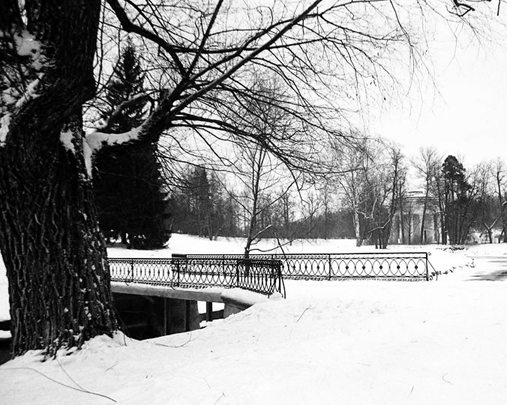
\includegraphics[width=0.45\textwidth]{thres/winter_o}}
\qquad
  \subfloat[Imagen binaria obtenida a trav\'es de un m\'etodo del valor umbral]{\label{fig:thres1}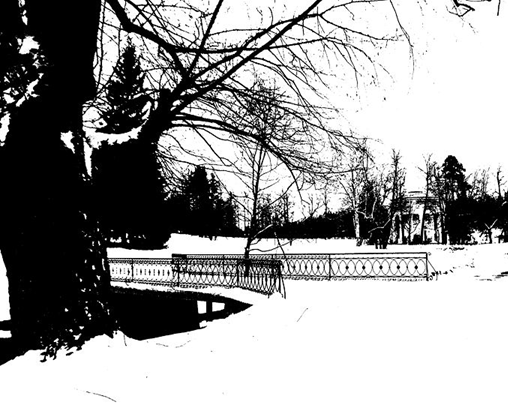
\includegraphics[width=0.45\textwidth]{thres/winter_thres}}
  \caption[Imagen en escala de grises antes y despu\'es de aplicar un m\'etodo del valor umbral ]{Imagen en escala de grises antes y despu\'es de 
    aplicar un m\'etodo del valor umbral. Las im\'agenes fueron tomadas de \cite{web:thresholding}}
  \label{fig:thres1}
\end{figure}

\section{Transformada de Distancia}
\label{sec:dt}

Una transformada de distancia o mapa de distancias es una representaci\'on de
una imagen digital, en la cual a cada pixel de la imagen le corresponde
un valor que indica la distancia entre ese pixel y el pixel m\'as cercano que pertenezca
al fondo de la imagen. Se calcula a partir de una imagen binaria, que consista
en p\'ixeles de objeto y p\'ixeles de fondo. La imagen que se obtiene corresponde a
una especie de representaci\'on en escala de grises del primer plano de la imagen
binaria (conformado por los objetos).\\
El valor mapeado para cada pixel, depende directamente de la funci\'on de distancia,
que define el patr\'on de medici\'on de distancia entre p\'ixeles de la imagen. Existen
diversas funciones de distancia tales como: \emph{Manhattan},
\emph{tablero de ajedrez}, \emph{Euclidiana}, \emph{Chamfer 3-4} y \emph{Octogonal}, 
\cite[p.363]{dtresearch}. As\'i mismo, existen muchas otras funciones de
distancia, normalmente derivadas de las anteriormente mencionadas.
En la Figura \ref{fig:dtexamples}, se muestra el resultado de aplicar 
diferentes funciones de distancia a una imagen que contiene un punto en el centro,
rodeado por un fondo blanco.

\begin{figure}[h t b p ! H]
 \centering
   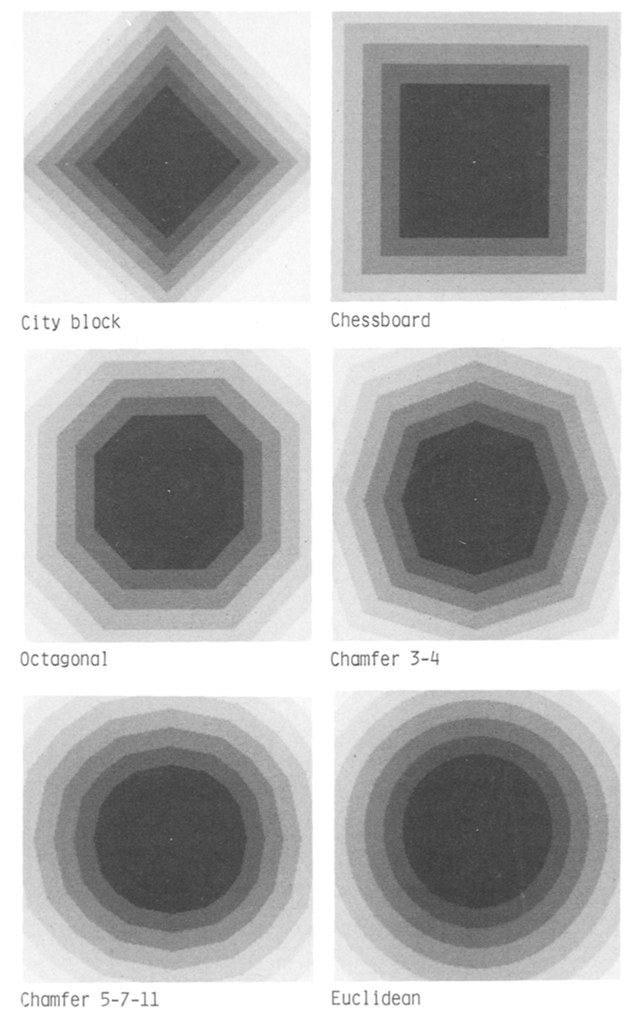
\includegraphics[scale=0.4]{dt/dtref}
 \caption[Distancias a partir de un punto para seis transformadas de distancia]{ 
   Distancias a partir de un punto para seis transformadas de distancia. Mientras 
   m\'as claro es el color, m\'as larga es la distancia \cite[p.365]{dtresearch}}
 \label{fig:dtexamples}
\end{figure}

Como se indica en \cite{dtresearch2}, las transformadas de distancia juegan un rol
central en la comparaci\'on de im\'agenes binarias, particularmente aquellas
resultantes de t\'ecnicas de detecci\'on de caracter\'isticas locales, tales 
como detecci\'on de contornos o detecci\'on de esquinas.
Las transformadas de distancia pueden ser interpretadas, tambi\'en, como
topograf\'ias de islas, donde la etiqueta o valor de cada pixel indica la altura o 
profundidad de la regi\'on. De esta forma, se pueden detectar crestas y picos, 
que constituyen la base principal de met\'odos sencillos para encontrar el 
esqueleto topol\'ogico de objetos en im\'agenes, tal como se explica en \cite[p.237]{ridgedt}.
Las transformadas de distancias son tambi\'en herramientas muy \'utiles para el 
mejoramiento de la eficiencia de algoritmos de morfolog\'ia, tales como: 
\emph{reducci\'on de contornos} y \emph{expansi\'on de contornos}.\\

\section{\emph{Skeletonization}}
\label{sec:skeletonization}

Un esqueleto topol\'ogico es una representaci\'on compacta y simple de un objeto, que
consiste en una versi\'on reducida o delgada del mismo, que es equidistante a sus bordes, 
y que preserva muchas de las caracter\'isticas topol\'ogicas y geom\'etricas de la
imagen original, tal como se explica en \cite{wikipedia:skeleton,ssm,augmented}. 
Por lo general, el esqueleto se define como el conjunto de los centros de los discos m\'aximos
contenidos en la imagen original, \cite{ssm,augmented}. Existen muchas otras definiciones diferentes,
que dependen, principalmente, de la forma en que el esqueleto es generado.
Independientemente de la definici\'on que se adopte, si los puntos pertenecientes al esqueleto
son calculados en relaci\'on con su distancia a los bordes originales del objeto, 
el esqueleto puede ser utilizado para reconstruir con exactitud la figura original.
La figura \ref{fig:genskeleton} presenta el esqueleto de una silueta de caballo, y la
imagen binaria a partir de la cual fue calculado el esqueleto.

\begin{figure}[h t b p ! H]
  \centering
  \subfloat[Imagen Binaria]{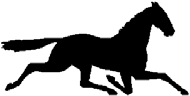
\includegraphics[scale=0.8]{skeleton/horsebinary}}
\qquad
  \subfloat[Esqueleto topol\'ogico]{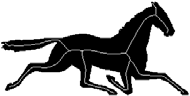
\includegraphics[scale=0.8]{skeleton/horseskeleton}}
  \caption[Imagen binaria y esqueleto topol\'ogico de una figura de caballo]{Imagen binaria de una figura de
caballo y su esqueleto. Im\'agenes tomadas de \cite{ssm}}
  \label{fig:genskeleton}
\end{figure}


Los esqueletos topol\'ogicos pueden ser categorizados en diferentes tipos.
Telea et al, \cite{augmented}, describen tres tipos de esqueleto de acuerdo a la forma en que
son calculados, tales como: \emph{esqueleto por reducci\'on morfol\'ogica}, 
\emph{esqueleto por m\'etodos geom\'etricos} y \emph{esqueleto por transformada de distancia}.
El m\'etodo de \emph{reducci\'on morfol\'ogica} consiste en la reducci\'on iterativa de los bordes
del objeto, identificando y marcando, capa por capa, aquellos puntos cuya remoci\'on no afecte
la topolog\'ia del objeto. Estos m\'etodos son sencillos, por lo general, aunque suelen requerir
heur\'isticas complejas para asegurar la conectividad del esqueleto, como se indica en
\cite{augmented}. En \cite{onepass} y \cite{thinning}, se describen dos enfoques paralelos
eficientes para garantizar la conectividad de esqueletos producidos a trav\'es 
\emph{reducci\'on morfol\'ogica}.\\
Los \emph{m\'etodos geom\'etricos} se centran en calcular el diagrama de Voronoi de una
representaci\'on poligonal de los bordes del objeto. El diagrama de Voronoi representa
el eje medio de los bordes. Tal como se asegura en \cite[p.251]{augmented}, estos m\'etodos
producen un esqueleto conectado y preciso, pero son muy complejos de implementar, requieren
una robusta discretizaci\'on de los bordes, y son computacionalmente costosos.\\
El tercer tipo comprende los m\'etodos que calculan el esqueleto a partir de 
la transformada de distancia. El enfoque com\'un consiste en encontrar los puntos cresta
y conectarlos, \cite{maxima, euclideancentre, ridgedt}. Por lo general, estos m\'etodos
pueden garantizar que los puntos esqueletos encontrados sean precisos y acertados, 
pero no la conectividad del esqueleto, ni su completitud.\\

El esqueleto topol\'ogico es una herramienta importante para la representaci\'on
y reconocimiento de objetos, en diferentes \'areas, tales como: visi\'on artificial,
an\'alisis de im\'agenes, y procesamiento de im\'agenes digitales, incluyendo 
reconocimiento \'optico de caracteres, reconocimiento de huellas digitales, inspecci\'on
visual, reconocimiento de patrones, compresi\'on de im\'agenes binarias y plegamiento
de prote\'inas, \cite{skprotein}.


\section{Ajuste de formas}
\label{sec:shapefitting}

El ajuste de formas (en ingl\'es \emph{shape matching}), es un problema
central en los sistemas de informaci\'on visual, visi\'on artificial, 
reconocimiento de patrones y rob\'otica, \cite{matchingbook}. Consiste
en identificar el \'area o contorno de una forma en espec\'ifico o de determinadas 
clases de formas en una imagen, y tiene un rol fundamental en la extracci\'on
de contenido en im\'agenes y en la recuperaci\'on de im\'agenes basada en contenido.
Tal como explica Veltkamp en \cite{matching2}, el ajuste de formas 
se ocupa de la transformaci\'on de una forma determinada y de la
medici\'on de su similitud con respecto a otra forma, utilizando
alguna medida de similitud o distancia entre formas.\\

El concepto de forma es abstracto. La mayor\'ia de los
enfoques en ajuste de formas definen las formas de manera 
geom\'etrica. Esta descripci\'on geom\'etrica puede 
consistir tanto en un conjunto de puntos, curvas, superficies,
s\'olidos, etc, como en un patr\'on geom\'etrico dispuesto de acuerdo
a alg\'un grupo de transformaciones geom\'etricas, en particular transformaciones
de semejanza (traslaci\'on, rotaci\'on y escala), tal como se indica en
\cite{matching2}. 

Por lo general, se utiliza un patr\'on geom\'etrico de forma, llamado
descriptor de forma, para representar la clase del objeto a ajustar.
Existen diferentes tipos de descriptores de forma, que se diferencian de acuerdo
al tipo de informaci\'on que los define y a la naturaleza del problema, (ver
Sec. \ref{sec:shapedesc}).\\

Se han desarrollado diferentes enfoques para el problema de ajuste de formas.
Esta secci\'on se centra en aquellos enfoques basados en geometr\'ia
computacional, dado que son los m\'as relacionados con el enfoque
seguido en este trabajo. La geometr\'ia computacional consiste en buscar y 
analizar algoritmos eficientes para resolver problem\'as geom\'etricos.
En \cite{matchingbook}, Veltkamp y Hagedoorn mencionan diferentes
enfoques de ajuste de formas tales como: poda de \'arboles, la transformada
de Hough generalizada, el m\'etodo de alineaci\'on, estad\'isticas,
modelos deformables, relajaci\'on de etiquetas, descriptores de Fourier,
transformada \'ondula y redes neurales. As\'i mismo, categorizan las 
t\'ecnicas de ajuste de forma en dos grupos principales:
\emph{transformadas de imagen global} y \emph{m\'etodos de objetos globales}.\\

El grupo de \emph{transformadas de imagen global} se refiere a las 
t\'ecnicas que ``transforman la imagen de informaci\'on de color en
el dominio espacial a variaci\'on de color en el dominio frecuencial'', 
\cite{matchingbook}. Estos enfoques no representan la forma expl\'icitamente 
para el ajuste,
sino que representan las transiciones de color o intensidad en
la imagen. Esto hace imposible medir las diferencias entre dos
im\'agenes en t\'erminos de formas, as\'i como comparar y ajustar
una forma a una parte espec\'ifica de la imagen.\\
Por otro lado, los \emph{m\'etodos de objetos globales} trabajan 
con \'areas completas de los objetos o con los contornos, y pueden
analizar secciones espec\'ificas de la imagen, en vez de requerir
el procesamiento de la imagen como un todo, tal como en las 
\emph{transformadas de imagen global}. En estos m\'etodos se requiere
que los objetos de la imagen est\'en completamente segmentados. Algunos
de estos m\'etodos son: \emph{m\'etodo de momentos}, donde los
objetos son descrito como un conjunto de momentos (posici\'on, \'area,
orientaci\'on, y otros par\'ametros) y se detecta la invariancia de 
momentos en los objetos; \emph{m\'etodo de ajuste modal}, donde 
se utilizan los bordes descritos con descriptores de Fourier; y
\emph{m\'etodo de curvatura de espacio escalado}, donde se utiliza 
un espacio escalado y una parametrizaci\'on del contorno de los objetos.\\

Veltkamp describe en \cite{matching2} diversas formas de las cuales
puede ser estudiado el problema de ajuste de formas, dados
dos patrones de forma y una medida de similitud. Estos son:


\begin{itemize}
\item \textbf{Problema computacional:} Computa la disimilitud entre
dos patrones de formas.
\item \textbf{Problema de decisi\'on: }
  \begin{itemize}
  \item  Para un umbral determinado, decidir si la disimilitud es 
    m\'as peque\~na que el umbral
  \item Para un umbral determinado, decidir si existe una transformaci\'on
    tal que la disimilitud entre el patr\'on transformado y el otro
    patr\'on es menor que el umbral
  \end{itemize}
 
\item \textbf{Problema de optimizaci\'on: } Encuentra la transformaci\'on
que minimiza las disimilitud entre el patr\'on transformado y otro patr\'on.
\end{itemize}

Existe un enfoque de ajuste de formas muy estudiado, basado en optimizaci\'on,
que se conoce como Modelos de Contornos Activos, en particular el modelo de \emph{snakes}, 
el cual inspir\'o gran parte del enfoque de ajuste de formas presentado en este trabajo, (Ver
Sec. \ref{sec:metfit}). En \cite{snakes}, un \emph{snake} es definido como
un \emph{spline} minimizador de energ\'ia, que es guiado por fuerzas de restricciones
externas e influenciado por fuerzas internas de la imagen que lo empujan
hacia elementos caracter\'isticos tales como: l\'ineas y contornos.
Se dice que los \emph{snakes} son modelos de contornos activos, debido a que
se pliegan a contornos cercanos y los localizan con precisi\'on.\\
El modelo de \emph{snakes} se define como un \emph{spline} continuo y controlado que 
es restringido por fuerzas internas y externas de la imagen, llamadas energ\'ias.
La energ\'ia interna modela la resistencia del objeto a ser empujado por fuerzas externas
hacia direcciones inconsistentes, de acuerdo a la informaci\'on previa que se tiene sobre 
el objeto y la imagen, \cite{deformable}. En este caso, la energ\'ia interna impone una
restricci\'on de suavidad a trozos (``\emph{piecewise smoothness constraint}'', \cite{snakes}).
Esto significa que el contorno es empujado hacia elementos resaltantes de la imagen por las
fuerzas externas, mientras que el contorno en si mismo exhibe resistencia a ser deformado
en un curva no-suave. Como se explica en \cite{deformable}, las fuerzas de la imagen
empujan al \emph{snake} hacia salientes o caracter\'isticas resaltantes de la imagen como l\'ineas,
bordes y contornos subjetivos, mientras que las fuerzas externas de restricci\'on son responsables
por ubicar al \emph{snake} cerca del m\'inimo local deseado.\\

Dado estas definiciones, sea $M$ el modelo a deformar y $D$ el conjunto de datos, 
la energ\'ia total $E$ puede ser definida como:

$$E(M,D) = E_{ext}(M,D) + E_{int}(M,D)$$

donde $E_{ext}$ es la funci\'on de energ\'ia externa y $E_{int}$ la funci\'on
de energ\'ia interna. De esta manera, la t\'ecnica de optimizaci\'on se centra
en minimizar la funci\'on objetivo definida por la energ\'ia total.

\section{Descriptores de Forma}
\label{sec:shapedesc}

Un descriptor de forma es una abstracci\'on estructurada 
de una clase de formas, que las describe de manera 
geom\'etrica. Los descriptores de forma pueden ser tanto
fijos como variables. Los descriptores fijos son aquellos
que representan un conjunto previamente definido de formas, 
a manera de plantillas. Los descriptores variables definen
una serie de par\'ametros para representar la forma. Dependiendo
de los valores as\'ignados a los diferentes par\'ametros, se obtienen
diferentes variaciones de formas, que igualmente pertenecen al tipo
o clase de formas representadas por el descriptor. 
Los descriptores o modelos de formas han sido ampliamente utilizados para
interpretar de manera robusta objetos complejos, \cite{wormparam}. 

Latecki et al \cite{shapenonrigid}, separan los descriptores en tres
categor\'ias principales:

\begin{itemize}
\item \textbf{Descriptores basados en contornos: } El contorno de un
objeto determinado es mapeado a alg\'un tipo de representaci\'on, a partir de la cual
se deriva un descriptor de forma.
\item \textbf{Descriptores basados en im\'agenes: } El c\'alculo del descriptor
de forma se basa en agrupar el valor de los p\'ixeles de una imagen digital
que contiene la silueta del objeto, a partir de los cuales se construye un vector
descriptivo de par\'ametros variables.
\item \textbf{Descriptores basados en el esqueleto topol\'ogico: } Luego de que
el esqueleto de la imagen es calculado, este es mapeado a una estructura 
de \'arbol que conforma el descriptor de forma. La disimilitud entre formas
es calculado a trav\'es de alg\'un algoritmo de grafos.
\end{itemize}

Considerando que, b\'as\'icamente, los descriptores de forma son intentos de cuantificar
una forma en t\'erminos f\'acilmente abstraibles por la mente humana, \cite[p.1]{desclecture},
cualquier tipo de representaci\'on geom\'etrica que cubra los elementos o propiedades que
quieren ser descritos en una forma, puede ser usado como descriptor. En \cite{desclecture},
se cubren los descriptores de forma basados en regiones. Estos son todos aquellos que describen
una forma en base a las propiedades geom\'etricas y num\'ericas de la regi\'on que esta cubre.
Algunos descriptores simples son mencionados, tales como: el \'area, el per\'imetro,
compacidad (no-compacidad), circularidad (no-circularidad), excentricidad, elongaci\'on,
rectangularidad y orientaci\'on. Cualesquiera combinaciones de estas propiedades de una forma
son \'utiles para describirla de manera b\'as\'ica. Se mencionan tamb\'ien otras propiedades
m\'as complejas para mejorar la precisi\'on del descriptor, como lo son: la envoltura conexa, 
puntos extremos, perfiles, momentos y perfil de momentos.\\
La envoltura convexa mide la cantidad de concavidades que presenta la forma.
El descriptor de puntos extremos se centra en encontrar los puntos l\'imite de una forma. Esto puede ser, 
tanto una representaci\'on simple como el \emph{rect\'angulo delimitador}, como una
representaci\'on m\'as poderosa, como lo es el encontrar los ocho puntos extremos de la figura
como lo son: norte, nor-oeste, oeste, sur-oeste, y as\'i sucesivamente. El descriptor por
perfiles, se basa en el n\'umero de p\'ixeles que la forma presenta en un direcci\'on determinada,
ya sea vertical, horizontal o diagonal. El descriptor por momentos, se basa en el c\'alculo
de momentos estad\'isticos, y el descriptor de perfil de momentos, es una combinaci\'on de
los \'ultimos dos.\\


Un descriptor puede o no permitir la reconstrucci\'on de la forma original que
describen, dependiendo de las propiedades que controlan y miden.
En \cite{wormparam}, se presenta un m\'etodo entrenable para representaci\'on
de formas, que permite capturar autom\'aticamente las propiedades invariables
de una clase de formas y proveer un descripci\'on param\'etrica compacta. Este
m\'etodo fue aplicado en gusanos, obteniendo un descriptor que reconstruye
formas de gusanos con diferentes flexiones, dependiendo de los valores
as\'ignados a los par\'ametros que la definen.

\section{\emph{Splines}}
\label{sec:splines}

El t\'ermino \emph{spline}, de la forma en que se utiliza en este trabajo, se refiere en general 
a una curva definida a trozos mediante polinomios. Los \emph{splines} han sido ampliamente
utilizados en los subcampos de las ciencias de la computaci\'on, por la simplicidad de su 
construcci\'on, la facilidad y precisi\'on de su evaluaci\'on, y su capacidad para aproximar
formas o figuras complejas, como se explica en \cite{web:splines}. 
La representaci\'on de una curva continua es particularmente apropiada para problem\'as
como: detecci\'on de contornos, ajuste de superficies y t\'ecnicas de multi-resoluci\'on.
Es igualmente \'util para muchos otros problem\'as en visi\'on artificial como: flujo \'optico,
reconstrucci\'on de superficies y recobramiento de iluminaci\'on y color, \cite[821]{splinespap}.\\

Los \emph{splines} reciben nombres diferentes dependiendo de diversas condiciones.\\
Un tipo de \emph{spline}, muy com\'unmente utilizado en reconocimiento de objetos, es
el \emph{spline de Hermite}. Este, es un \emph{spline} de tercer grado, que se expresa
 utilizando polinomios de Hermite, para representar cada una de las porciones individuales
del polinomio.
Diversos m\'etodos han sido desarrollados para ajustar estos \emph{splines} a un conjunto
de puntos tales como: \emph{spline} cardinal, \emph{splines} de Catmull-Rom y \emph{splines} de
Kochanek-Bartels. Todos estos permiten construir una curva suave que pasa por cada punto
del conjunto. De esta manera, dados una serie de puntos que pertenecen, digamos, al contorno de 
un objeto, una figura suave puede ser calculada, que modele la forma definida por el objeto.
Los \emph{splines} de Hermite proveen una cantidad de ventajas que lo hacen \'utiles 
en el procesamiento de im\'agenes, como se menciona en \cite{splinespap}. Primero,
los \emph{splines} de Hermite son, por lo general, curvas suaves y que tienden muy poco
a oscilar, al contrario de los polinomios de orden superior. Adem\'as, estos \emph{splines} son
continuos en todas partes, en contraste a los polinomios encontrados por aproximaciones locales.
que puede producir discontinuidades fuertes en la 
conexi\'on de regiones. Finalmente, tienen la ventaja de poder ser evaluados f\'acilmente.